\documentclass[a4paper,11pt]{article}
%\usepackage[utf8x]{inputenc}
\usepackage{latexsym}
\usepackage[spanish]{babel}
\usepackage[utf8]{inputenc}
\usepackage[T1]{fontenc}
\usepackage{graphicx} 
\usepackage[colorlinks=true,linkcolor=black,urlcolor=black]{hyperref}
\usepackage{listings}
\usepackage{xcolor} %para darle color a los codigos
\usepackage{lmodern} %para agregarle bold a las letras ttfamily
% para cambiar los margenes
\usepackage{anysize}
\marginsize{3cm}{3cm}{2cm}{2cm} 

\definecolor{gray97}{gray}{.9}
\definecolor{gray45}{gray}{.45}
%% Configura las opciones de ``listings''
\lstset{ frame=Ltb,
framerule=0pt,
aboveskip=0.5cm,
framextopmargin=3pt,
framexbottommargin=3pt,
framexleftmargin=0.4cm,
framesep=0pt,
rulesep=.4pt,
backgroundcolor=\color{gray97},
rulesepcolor=\color{black},
%
stringstyle=\ttfamily,
showstringspaces = false,
basicstyle=\small\ttfamily,
commentstyle=\color{gray45},
keywordstyle=\bfseries,
%
numbers=left,
numbersep=15pt,
numberstyle=\tiny,
numberfirstline = false,
breaklines=true,
}

\lstdefinelanguage{VHDL}{
  morekeywords={
    library,use,all,entity,is,port,in,out,end,architecture,of,
    begin,and,case,if,else,when,while,process,loop,for,then,elsif,signal,
    variable,constant,with,select,ENTITY,SIGNAL,PROCESS,WAIT,EVENT,AND,
    USE,ALL,IS,PORT,IN,OUT,END,ARCHITECTURE,OF,BEGIN,CASE,IF,ELSE,WHEN
  },
  morecomment=[l]--
}
\lstdefinelanguage{{[x86masm]Assembler}}{
  morekeywords={
    LOAD,STORE,ADD
  },
  morecomment=[l];
}

\colorlet{keyword}{blue!100!black!80}
\colorlet{comment}{green!90!black!90}
\lstdefinestyle{vhdl}{
  language     = VHDL,
  basicstyle   = \ttfamily,
  keywordstyle = \color{keyword}\bfseries,
  commentstyle = \color{comment}
}



%opening
\title{\vspace{6cm} Microprocesadores en VHDL, aspectos prácticos \\ 
%\large Circuitos Digitales y Microprocesadores \\ 
\large Codiseño Software Hardware \\ 
\large Departamento de electrotécnia \\
\large Universidad Nacional de la Plata
}
\author{ Ing. Eduardo Kunysz}
\begin{document}
\thispagestyle{empty} %Para que no numere esta página

\begin{center}

\includegraphics[width=1\textwidth]{graficos/encabezado.jpg} 
\hspace{-1cm}
\begin{tabular}{c} 
 {\it \bf Facultad de Ingeniería -- Universidad Nacional de La Plata} \\ 
\vspace{0.2cm} {\it  Departamento de Electrotecnia. CeTAD.} 
\end{tabular}
\end{center}
\begin{table}[h]
\hspace{1.3cm}
\begin{tabular}{p{12cm}}
\hline \\[1cm]
\vspace{5cm}
\begin{center}
\LARGE \textbf{Microprocesadores en VHDL,\\
aspectos prácticos}
\\[2cm] 
\end{center}

\end{tabular}

\end{table}
\begin{center}
%\large \textbf{Cátedra de Circuitos Digitales y Microprocesadores}
\large \textbf{Cátedra de Codiseño Software Hardware}
\end{center}
\begin{center}
 \large \textbf{Versión 0.2}            
\end{center}


%\maketitle
\vspace{8cm}
\begin{flushright}
\large \textbf{Autor: Ing. Eduardo J. Kunysz}
\end{flushright}
\newpage
\thispagestyle{empty}
\begin{abstract}
El siguiente artículo tiene por objetivo describir las herramientas de descripción de hardware mediante VHDL con la finalidad de poder
desarrollar de forma conceptual y práctica un uProcesador básico con fines didácticos y educativos. 

En la primer parte se hace un breve resumen de algunos conceptos básicos de VHDL. En la segunda parte se ven algunos módulos
que forman parte de un microprocesador, en la tercer parte se implementa y simula un microprocesador sencillo.
\end{abstract}
\normalsize
\newpage
\setcounter{page}{1}
\tableofcontents

\section{VHDL}
\subsection{Introducción}
VHDL es un lenguaje de descripción de circuitos electrónico digitales que utiliza distintos niveles de abstracción. Creado en 1980 por 
el DoD\footnote{\textit{Department of Defense}} de Estados Unidos y el IEEE. Acrónimo de ``VHSIC\footnote{\textit{Very High Speed 
Integrated Circuit}} Hardware Description Language''.

El lenguaje tiene las siguientes características:
\begin{itemize}
 \item Los diseños pueden descomponerse jerárquicamente.
 \item Cáda elemento del diseño tiene una interfaz bien definida (para conectarla a otros elementos) como una especificación de 
comportamiento precisa (para simularla)
 \item El comportamiento puede ser especificado por un algoritmo o bien por una estructura de hardware real.
 \item La concurrencia, temporización y señales de reloj pueden ser todas modeladas.
 \item La operación lógica y comportamiento de temporización de un diseño pueden simularse.
\end{itemize}

VHDL comenzó como un lenguaje de modelado y documentación. Si bien esto fue una innovación importante, el salto cuántico lo obtuvo con 
el desarrollo de herramientas de síntesis VHDL. Estos programas tienen la capacidad de crear circuitos lógicos a partir de su descripción
en hardware. Con VHDL se puede simular y sintetizar cualquier circuito combinacional simple hasta un ``microprocesador completo''.

VHDL en si no es un lenguaje de programación, por lo tanto no alcanza con conocer su sintaxis. Para diseñar en VHDL hay que:
\begin{itemize}
 \item Pensar en puertas y biestables, no en variables o funciones.
 \item Evitar bucles combinacionales y relojes condicionados.
 \item Saber qué parte del circuito es combinacional y cuál secuencial.
\end{itemize}

El objetivo final de escribir código en VHDL es poder diseñar circuitos que se puedan implementar en circuitos integrados de lógica
programable como CPLD o FPGA's.

\subsection{Estructura de programa}
Los archivos generados en VHDL (extensión .vhd) tienen la descripción del circuito que se quiere implementar. Viéndolo a nivel macro, 
nos encontraremos con dos grandes bloques como se observa en la Figura \ref{vhdlbloque}

\begin{figure}[h]
  \centering
    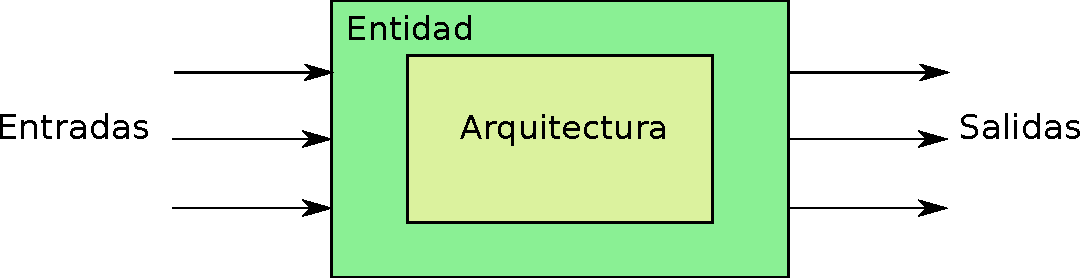
\includegraphics[width=.85\textwidth]{graficos/vhdl.pdf}
  \caption{Estructura VHDL}
  \label{vhdlbloque}
\end{figure}

\subsubsection{Entidades (Entity)}
La entidad describe únicamente la forma externa del circuito. Es el lugar donde se enumeran las entradas y salidas del diseño.
Podríamos imaginarnos a una entidad como un símbolo esquemático de un diagrama electrónico, el cual describe las conexiones del 
dispositivo hacia el resto del diseño.
La Figura \ref{entidad} describe gráficamente este concepto.

\begin{figure}[h]
  \centering
    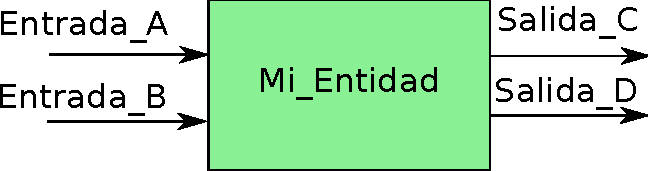
\includegraphics[width=.5\textwidth]{graficos/entidad.pdf}
  \caption{Entidad VHDL}
  \label{entidad}
\end{figure}


\begin{lstlisting}[style=vhdl]
entity Mi_Entidad is
     port (Entrada_A,Entrada_B : in  bit;
           Salida_A,Salida_B   : out bit)
end Mi_Entidad
\end{lstlisting}

\subsubsection{Arquitectura (Architecture)}
La arquitectura es una detallada descripción del comportamiento o estructura interna del módulo. Si vemos a la entidad como una caja 
negra en la que se enumeran las interfaces de conexión, la arquitectura representa la estructura interna de dicha caja.

\begin{lstlisting}[style=vhdl]
architecture Nombre_arquitectura of Mi_entidad is
--declaracion de senales;
begin
--Sentencias concurrentes (combinacionales)
--Sentencias secuenciales
   process (lista de sensibilidad)
   --declaracion de variables;
   begin
     --sentencias
   end process;
end nombre_arquitectura
\end{lstlisting}

\subsubsection{Identificadores}

\paragraph{Constant}
Los objetos de esta clase tienen un valor inicial que es asignado de
forma previa a la simulación y que no puede ser modificado durante ésta.
\begin{lstlisting}[style=vhdl]
 constant identificador: tipo:= valor;
\end{lstlisting}

\paragraph{Variable}
Los objetos de esta clase contienen un único valor que puede ser
cambiado durante la simulación con una sentencia de asignación. Las variables
generalmente se utilizan como índices, principalmente en instrucciones de bucle, o
para tomar valores que permitan modelar componentes. Las variables NO
representan conexiones o estados de memoria.
\begin{lstlisting}[style=vhdl]
 variable identificador: tipo [:= valor];
\end{lstlisting}

\paragraph{Signals}
Los objetos de esta clase contienen una lista de valores que incluye el
valor actual y un conjunto de valores futuros. Se las puede ver como los
``cables'' de interconexión de elementos. Las señales representan elementos de
memoria o conexiones y sí pueden ser sintetizadas. Los puertos de una entidad son
implícitamente declarados como señales en el momento de la declaración, ya que
estos representan conexiones. También pueden ser declaradas en la arquitectura
antes del BEGIN, lo cual nos permite realizar conexiones entre diferentes módulos.
\begin{lstlisting}[style=vhdl]
 signal identificador: tipo;
\end{lstlisting}

\subsubsection{Tipos y constantes}

Todas las señales, variables y constantes en un programa VHDL deben tener un ``tipo''
asociado. El tipo especifica el conjunto o intervalo de valores que el objeto puede tomar.
y también hay típicamente un conjunto de operadores (suma, ANO, etc.) asociados con un tipo dado.

A continuación se describirán algunos de los tipos mas utilizados:

\paragraph{BIT}
Puede tomar los valores ``0'' y ``1''.

\paragraph{BIT\_VECTOR}
Agrupación de bits. Por ejemplo:

\begin{lstlisting}[style=vhdl]
signal salida : BIT_VECTOR (0 to 3);
salida <="1000";
\end{lstlisting}

esto significa que:

salida(0)=``1''

salida(1)=``0''

salida(2)=``0''

salida(3)=``0''

\paragraph{INTEGER}
A veces utilizado para índicesde loops, constantes, valores genéricos, etc.

\paragraph{BOOLEAN}
Puede tomar los valores ``true'' o ``false''

\paragraph{STD\_LOGIC}
Los dos valores del tipo ``Bit'' no alcanzan para definir todos los estados que puede tomar una señal digital.
No es un tipo propio de VHDL, es un tipo definido en la librería IEEE.standard\_logic\_1164.

La tabla \ref{std_logic} describe los posibles valores que pueden tomar.

\begin{table}[!hbt] 
\centering
 \begin{tabular}{|c|c|}
\hline
U & No inicializado, valor por defecto. \\ \hline
X & Desconocido fuerte, salida con múltiples fuentes en corto \\ \hline
0 & Salida de una puerta con nivel lógico bajo \\ \hline
1 & Salida de una puerta con nivel lógico alto \\ \hline
Z & Alta Impedancia \\ \hline
W & Desconocido débil, terminación de bus \\ \hline
L & 0 débil, resistencia de pull-down \\ \hline
H & 1 débil, resistencia de pull-up \\ \hline
\end{tabular}
  \caption{Valores de Std\_Logic}
  \label{std_logic}
  
\end{table}      

\paragraph{STD\_LOGIC\_VECTOR}
Se utiliza para describir buses, es un array de ``Std\_Logic''.

\subsubsection{Operadores}
Los operadores integrados para los tipos ``integer'' y ``boolean'' se enumeran en la tabla \ref{operadores}.

\begin{table}[!hbt] 
\centering
 \begin{tabular}{|c|c|c|c|}
\hline
\multicolumn{2}{|c|}{\textbf{Operadores Integer}} & \multicolumn{2}{|c|}{\textbf{Operadores Boolean}}\\ \hline
+   & Suma               & and   & AND  \\ \hline
-   & Resta              & or    & OR   \\ \hline
*   & Multiplicación     & nand  & NAND \\ \hline
/   & División           & nor   & NOR  \\ \hline
mod & División entera    & xor   & XOR  \\ \hline
rem & Residuo            & xnor  & XNOR \\ \hline
abs & Valor absoluto     & not   & NOT  \\ \hline
**  & Exponencial        &       &      \\ \hline


\end{tabular}
  \caption{operadores}
  \label{operadores}
  
\end{table}    

\subsection{Descripción de comportamiento}
\subsubsection{PROCESS}
Un PROCESS es una sentencia concurrente, esto significa que si tenemos varios PROCESS (y se dan las condiciones adecuadas), los mismos 
se ejecutarán al mismo tiempo. No obstante las sentencias que hay dentro del PROCESS se ejecutan de forma secuencial. Es la única forma
que tenemos en VHDL de ejecutar algo en forma secuencial.

Por lo tanto se puede decir que una estructura secuencial va en el interior de un PROCESS.

La estructura genérica de esta sentencia es:

\begin{lstlisting}[style=vhdl]
 PROCESS [lista de sensibilidad]
       --declaracion de variables
     BEGIN
       --sentencias secuenciales
     END PROCESS;
\end{lstlisting}

La lista de sensibilidad \footnote{La lista de sensibilidad solo funciona en simulación, cuando se implemente el hardware, 
se deben utilizar otras técnicas} es una serie de señales que, al cambiar de valor, hacen que se ejecute el PROCESS.

Un ejemplo sería:

\begin{lstlisting}[style=vhdl]
 PROCESS(signal1, signal2)
     ...
\end{lstlisting}

\subsubsection{WAIT}
Se utiliza para reemplazar la lista de sensibilidad

\begin{lstlisting}[style=vhdl]
 wait on signal_list;
 wait for time_expression;
 wait until condition;
\end{lstlisting}

Los eventos sobre las señales (‘EVENT) nos indican cuando ocurre un cambio en la señal
\begin{lstlisting}[style=vhdl]
signal'event
signal'last_event
signal'last_value
\end{lstlisting}


\subsubsection{IF – THEN – ELSE}
Sólo son aplicables dentro de un process
\begin{lstlisting}[style=vhdl]
if condicion then
   ...
   --sentencias secuenciales
elsif otra_condicion then
   ...
   --sentencias secuenciales
else
   ...
   --sentencias secuenciales
end if;
\end{lstlisting}

\subsubsection{CASE – WHEN} 
Sólo son aplicables dentro de un process
\begin{lstlisting}[style=vhdl]
case expresion is
   when alternativa_l =>  ... --sentencias sec.
   ...
   when alternativa_n =>  ... --sentencias sec.
   when others =>         ... --sentencias sec.
end case;
\end{lstlisting}

\subsubsection{FOR – LOOP}
Sólo son aplicables dentro de un process
\begin{lstlisting}[style=vhdl]
for loop_var in range loop
    ... --sentencias secuenciales
end loop; 
\end{lstlisting}

\subsubsection{WHILE – LOOP}
Sólo son aplicables dentro de un process
\begin{lstlisting}[style=vhdl]
 while condicion loop
    ... --sentencias secuenciales
end loop;
\end{lstlisting}

\subsubsection{WHEN – ELSE}
Sólo son aplicables dentro de un process
\begin{lstlisting}[style=vhdl]
 Signal_name <= valor_1 when condicion1 else
                valor_2 when condicionn2 else
                ...
                valor_i when condicioni else
                otro_valor;
\end{lstlisting}

\subsubsection{WITH – SELECT – WHEN}
Sólo son aplicables dentro de un process
\begin{lstlisting}[style=vhdl]
 with identificador select
 Signal_name <= valor_1    when valor_identificador1,
                valor_2    when valor_identificador2,
                ...
                valor_i    when valor_identificadori,
                otro_valor when others;

\end{lstlisting}

\section{Módulos digitales utilizando VHDL}
\subsection{Compuertas básicas}
El primer ejemplo consiste en una simple red de compuertas. La figura \ref{compuertas} muestra el circuito a describir.

\begin{figure}[h]
  \centering
    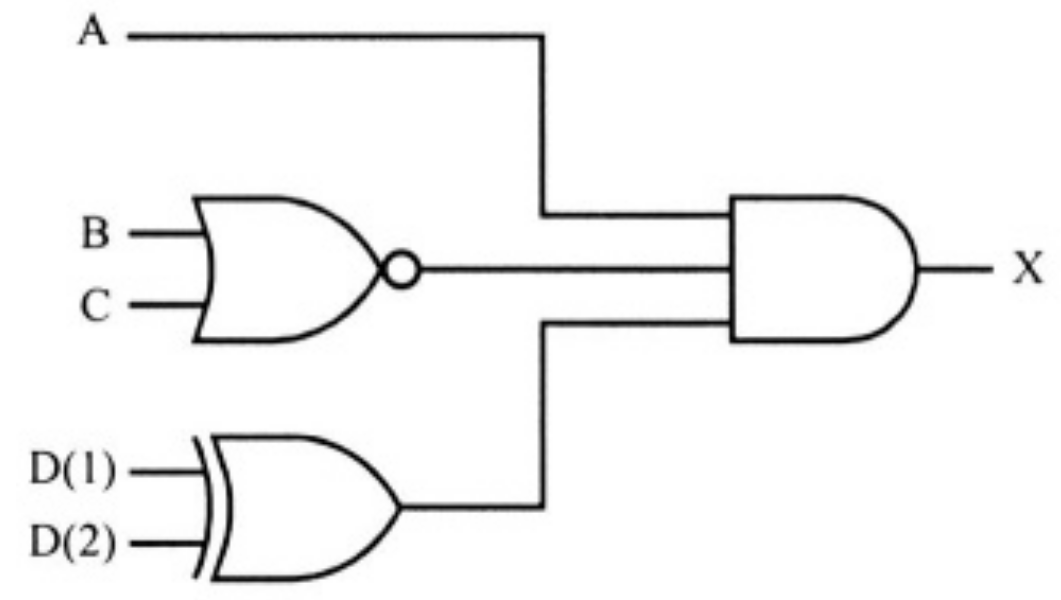
\includegraphics[width=.6\textwidth]{graficos/compuertas.png}
  \caption{Circuito digital basico basado en compuertas lógicas}
  \label{compuertas}
\end{figure}

\begin{lstlisting}[style=vhdl, basicstyle=\footnotesize\ttfamily]
--Se incluyen las librerias estandares de logica y tipos de datos
LIBRARY IEEE;
USE IEEE.STD_LOGIC_1164.ALL;

-- Normalmente el nombre de la entidad coincide con el nombre del archivo
-- Ports: Se declaran las entradas y salidas al modulo
ENTITY gate_network IS  
       PORT(A,B,C :IN STD_LOGIC;
            -- Arreglo de 2 bits
            D     :IN STD_LOGIC_VECTOR(1 DOWNTO 0);
            -- Señal de salida
            X     :OUT STD_LOGIC);
END gate_network;

-- Comienza la descripcion interna del modulo
ARCHITECTURE behavior OF gate_network IS
BEGIN                    --Sentencias concurrentes
            X <= A AND NOT( B OR C ) AND ( D( 1 ) XOR D( 2 ) );
END behavior;

            
\end{lstlisting}

\subsection{Modelo de Flip-Flops y Registros}
En el siguiente ejemplo se describirán algunas arquitecturas de flip-flops en VHDL. 
A diferencia de los dispositivos de hardware combinacionales anterior, un flip-flop sólo puede ser 
sintetizado dentro de un proceso. En VHDL ``Clock’EVENT'' es una condición verdadera siempre que 
la señal de clock cambie.

El flanco positivo se selecciona mediante `` Clock’EVENT AND clock=’1’ ''

El flanco negativo se selecciona mediante `` Clock’EVENT AND clock=’0’ ''

Para los siguientes ejemplos, la estructura del Entity y del Architecture es idéntica, sólo cambia 
el proceso interno, se definirá como puerto de salida distintos Q:

\begin{lstlisting}[style=vhdl, basicstyle=\footnotesize\ttfamily]
LIBRARY IEEE;
USE IEEE.STD_LOGIC_1164.ALL;
ENTITY DFFs IS
       PORT( D, Clock, Reset, Enable : IN STD_LOGIC;
             Q1, Q2, Q3, Q4          : OUT STD_LOGIC );
       END DFFs;
ARCHITECTURE behavior OF DFFs IS
       BEGIN 
         PROCESS
         ....
         END PROCESS;
       END behavior;
\end{lstlisting}

El flip flop de la figura \ref{ff1} es del tipo D disparado por flanco positivo
y para su implementación se utiliza WAIT para evitar el uso de listas de sensibilidad.

\begin{figure}[h!]
  \centering
    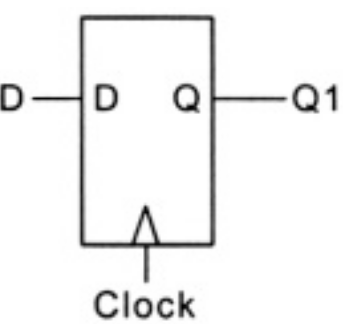
\includegraphics[width=.3\textwidth]{graficos/ff1.png}
  \caption{FF tipo D disparo por flanco positivo}
  \label{ff1}
\end{figure}

\begin{lstlisting}[style=vhdl, basicstyle=\footnotesize\ttfamily]
PROCESS
BEGIN
     WAIT UNTIL ( Clock 'EVENT AND Clock = '1');
           Q1 <= D;
END PROCESS;

\end{lstlisting}


El flip flop de la figura \ref{ff2} es del tipo D disparado por flanco positivo
con reset sincrónico.
\begin{figure}[h!]
  \centering
    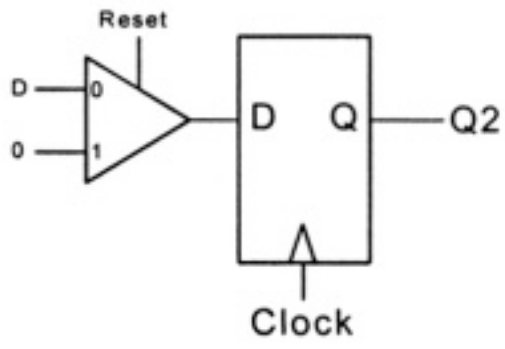
\includegraphics[width=.4\textwidth]{graficos/ff2.png}
  \caption{FF tipo D disparo por flanco positivo con reset sincrónico}
  \label{ff2}
\end{figure}

\begin{lstlisting}[style=vhdl, basicstyle=\footnotesize\ttfamily]
PROCESS
BEGIN
     WAIT UNTIL ( Clock 'EVENT AND Clock = '1');
           IF reset = '1' THEN
                Q2 <= '0';
           ELSE
                Q2 <= D;
           END IF;
END PROCESS;

\end{lstlisting}

El flip flop de la figura \ref{ff3} es del tipo D disparado por flanco positivo
con reset asincrónico. Para éste caso se utiliza la lista de sensibilidad para las
señales Reset y Clock.


\begin{figure}[h]
  \centering
    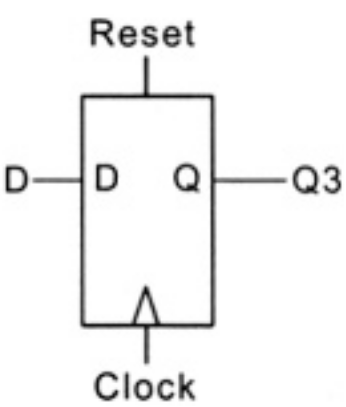
\includegraphics[width=.3\textwidth]{graficos/ff3.png}
  \caption{FF tipo D disparo por flanco positivo con reset asincrónico}
  \label{ff3}
\end{figure}


\begin{lstlisting}[style=vhdl, basicstyle=\footnotesize\ttfamily]
PROCESS (Reset,Clock)
BEGIN
     IF reset = '1' THEN
        Q3 <= '0';
     ELSIF ( clock 'EVENT AND clock = '1' ) THEN
        Q3 <= D;
     END IF;
END PROCESS;
\end{lstlisting}


El flip flop de la figura \ref{ff4} es del tipo D disparado por flanco positivo
con reset asincrónico y señal de habilitación.

\begin{figure}[h]
  \centering
    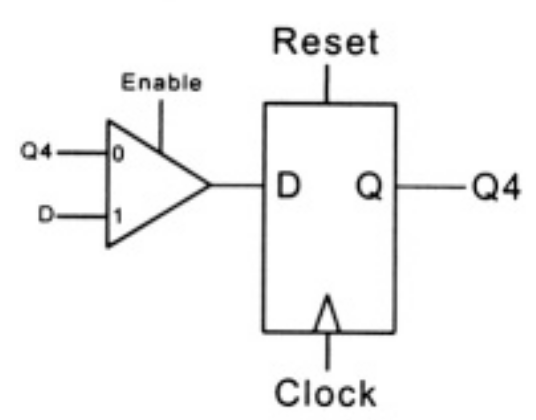
\includegraphics[width=.4\textwidth]{graficos/ff4.png}
  \caption{FF tipo D disparo por flanco positivo con reset asincrónico y habilitación}
  \label{ff4}
\end{figure}

\begin{lstlisting}[style=vhdl, basicstyle=\footnotesize\ttfamily]
PROCESS (Reset,Clock)
BEGIN
     IF reset = '1' THEN
        Q4 <= '0';
     ELSIF ( clock 'EVENT AND clock = '1' ) THEN
        IF Enable = '1' THEN
           Q4 <= D;
        END IF;
     EDN IF;
END PROCESS;
\end{lstlisting}

\subsection{Maquinas de estado sintetizadas en VHDL}
Una herramienta muy importante a la hora de trabajar en VHDL son las máquinas de estado. 
Cuando uno trabaja con circuitos digitales no hay que perder de vista que todos los procesos
que se ejecutan se realizan al mismo tiempo de forma concurrente (salvo dentro de los ``process``). 
La máquina de estados será una herramienta útil cuando se quiera realizar procesos secuenciales de forma ordenada.

En el siguiente ejemplo se describirá la máquina de Moore con tres estados, dos entradas y una salida.
El diagrama de dicha máquina se describe en la figura \ref{moore} 

\begin{figure}[h]
  \centering
    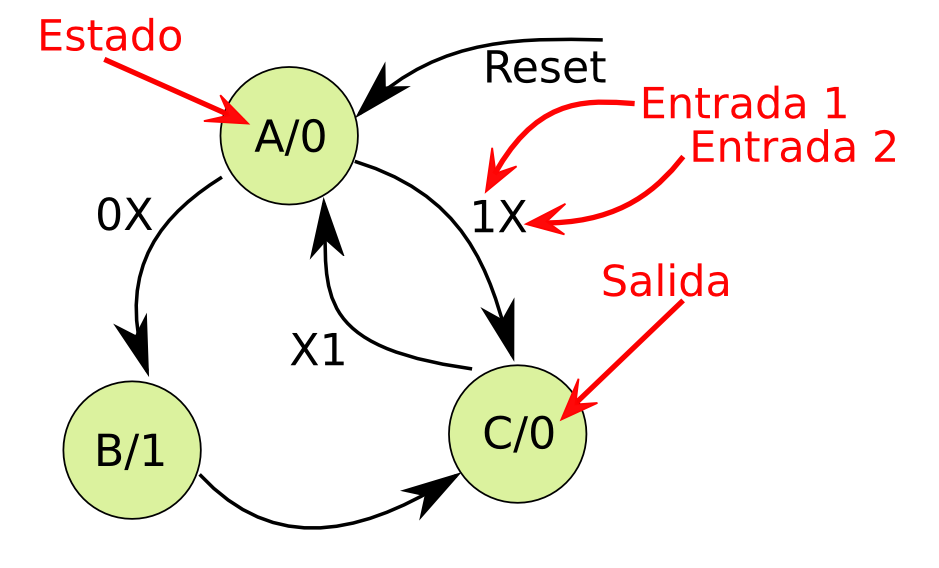
\includegraphics[width=.6\textwidth]{graficos/moore3.png}
  \caption{Máquina de estados de Moore}
  \label{moore}
\end{figure}

En VHDL, un tipo de datos enumerado se especifica, para el estado actual, con la instrucción ``TYPE''. 
Esto permite a la herramienta de síntesis asignar el valor de estado ``0'' o ``1''

Para evitar posibles problemas de ``timing``, señales externas de la maquina de estados desincronizadas, se deben
sincronizar pasando las señales a travez de flip-flops del tipo D, sincronizados con los relojes de la
máquina de estados.

\begin{lstlisting}[style=vhdl, basicstyle=\footnotesize\ttfamily]
LIBRARY IEEE;
USE IEEE.STD_LOGIC_1164.ALL;

ENTITY st_mach IS
   PORT( clk, reset      :IN STD_LOGIC;
         Input1, lnput2  :IN STD_LOGIC;
         Output1         :OUT STD_LOGIC);
END st_mach;

ARCHITECTURE A OF st_mach IS
--Enumerated Data Type for State
   TYPE STATE_TYPE IS ( state_A, state_B, state_C );
   SIGNAL state: STATE_TYPE;
BEGIN
   PROCESS ( reset, clk )
   BEGIN
      IF reset = '1' THEN   --Reset State
         state <= state_A;
      ELSIF clk 'EVENT AND clk = '1' THEN
         CASE state IS
            WHEN state_A =>
               IF Input1 = '0' THEN
                  state <= state_B;
               ELSE
                  state <= state_C;
               END IF;

            WHEN state_B =>
                  state <= state_C;

            WHEN state_C =>
               IF Input2 = '1' THEN
                  state <= state_A;
               END IF;

            WHEN OTHERS =>
                  state <= state_A;
         END CASE;
      END IF;
   END PROCESS;
   
   WITH state SELECT
      Output1 <= '0' WHEN state_A,
                 '1' WHEN state_B,
                 '0' WHEN state_C;
END A;
\end{lstlisting}

\subsection{Registro de 8 bits}
Uno de los elementos principales de todo procesador son los registros, el siguiente código 
en VHDL describe como realizar un registro de 8 bits.
port
\begin{lstlisting}[style=vhdl, basicstyle=\footnotesize\ttfamily]
LIBRARY IEEE;
USE IEEE.STD_LOGIC_1164.ALL;

ENTITY registro_8 IS
   PORT (clk, reset : in bit; 
         A          : in bit_vector(7 downto 0);
         B          : out bit_vector(7 downto 0));
   END registro_8;

ARCHITECTURE arch_reg OF registro_8 IS
BEGIN
   PROCESS(clk, reset)
   BEGIN
      IF reset=‘1’ THEN B<="00000000";
      ELSIF (clk'event and clk='1') THEN B<=A;
      END if;
   END PROCESS;
END arch_reg;
 
\end{lstlisting}

\subsection{Modelo de una ALU}
Hasta ahora hemos visto diversas estructuras y módulos simples en VHDL. Es hora de describir como 
implementar el elemento principal de todo microprocesador, la Unidad Aritmético Lógica. Para ello
realizaremos una ALU muy sencilla, que tome como entrada dos datos de 8 bits y mediante tres líneas
de control (Op\_codes) realice SUMA, RESTA, operaciones lógica AND, OR y adicionalmente le agregaremos
la opción de realizar corrimientos de datos a la salida mediante un registro de desplazamiento.
La figura \ref{alu} describe como será la estructura del código que implementaremos.
Las operaciones de los ``Op\_Codes'' se describen en la tabla \ref{aluopcodes}

\begin{figure}[h]
  \centering
    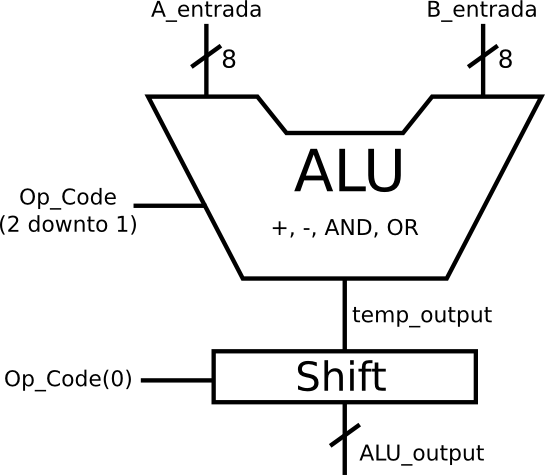
\includegraphics[width=.5\textwidth]{graficos/alu.png}
  \caption{ALU con Sumador/Restador y Desplazador}
  \label{alu}
\end{figure}

\begin{lstlisting}[style=vhdl, basicstyle=\footnotesize\ttfamily]
LIBRARY IEEE;
USE IEEE.STD_LOGIC_1164.ALL;
USE IEEE.STD_LOGIC_ARITH.ALL;
USE IEEE.STD_LOGIC_UNSIGNED.ALL;
ENTITY ALU IS
  PORT( Op_code              : IN STD_LOGIC_VECTOR( 2 DOWNTO 0 );
        A_entrada, B_entrada : IN STD_LOGIC_VECTOR( 7 DOWNTO 0 );
        ALU_output           : OUT STD_LOGIC_VECTOR( 7 DOWNTO 0 ) );
  END ALU;
ARCHITECTURE behavior OF ALU IS
   --Se describe lineas interna
   SIGNAL temp_output :STD_LOGIC_VECTOR( 7 DOWNTO 0 );
BEGIN
   PROCESS(Op_code, A_entrada, B_entrada)
   BEGIN
     CASE Op_code (2 downto 1) IS 
       WHEN "00"=>
        temp_output <= A_entrada + B_entrada;
       WHEN "01"=>
        temp_output <= A_entrada - B_entrada;
       WHEN "10"=>
        temp_output <= A_entrada AND B_entrada;
       WHEN "11"=>
        temp_output <= A_entrada OR B_entrada;
       WHEN OTHERS =>
        temp_output <= "00000000";
     END CASE

     --Operacion de desplazamiento (SHIFT)
     IF Op_code(0)='1' THEN 
       ALU_output <= temp_output(6 DOWNTO 0) & '0';
     ELSE 
       ALU_output <= temp_output;
     END_IF;
   END PROCESS;
END behavior;
\end{lstlisting}
\begin{table}[!hbt] 
\centering
 \begin{tabular}{|c|c|}
\hline
\textbf{Op\_Codes} & \textbf{Descripción} \\ \hline
000 & Suma \\ \hline
001 & Resta \\ \hline
010 & And \\ \hline
011 & Or \\ \hline
1XX & Desplazamiento \\ \hline
\end{tabular}
  \caption{Op\_codes del módulo ALU}
  \label{aluopcodes}
\end{table}  

\subsection{Modelo de una Memoria Simple}
Para explicar como se realiza una memoria realizaremos una memoria simple, con un
bus de 8 bits de datos, capacidad de 8 bytes por lo se podrá resolver con 3 bits de direccionamiento.
Para ello recurriremos a arreglos de ``standard logic vectors''. 
Esta aproximación es fácil de realizar en VHDL dado que el índice del arreglo genera 
la dirección. 
La figura \ref{ram} describe los puertos de conexión externa de la memoria

\begin{figure}[h]
  \centering
    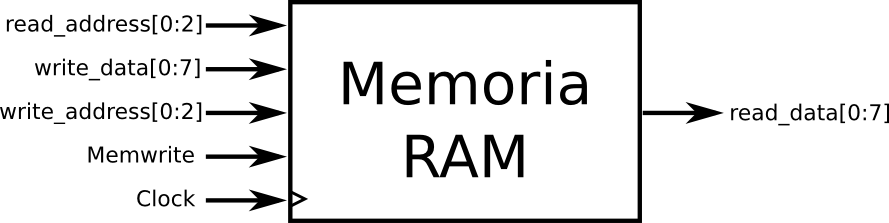
\includegraphics[width=.7\textwidth]{graficos/ram.png}
  \caption{Memoria RAM de 8 bits, capacidad 8 bytes}
  \label{ram}
\end{figure}
\begin{lstlisting}[style=vhdl, basicstyle=\footnotesize\ttfamily]
LIBRARY IEEE;
USE IEEE.STD_LOGIC_1164.ALL;
USE IEEE.STD_LOGIC_ARITH.ALL;
USE IEEE.STD_LOGIC_UNSIGNED.ALL;
ENTITY memory IS
  PORT( read_data     : OUT STD_LOGIC_VECTOR( 7 DOWNTO 0 );
        read_address  : IN STD_LOGIC_VECTOR( 2 DOWNTO 0 );
        write_data    : IN STD_LOGIC_VECTOR( 7 DOWNTO 0 ); 
        write_address : IN STD_LOGIC_VECTOR( 2 DOWNTO 0 );
        Memwrite      : IN STD_LOGIC;
        Clock         : IN STD_LOGIC );
  END memory;

ARCHITECTURE behavior OF memory IS
  --define un nuevo tipo como un arreglo de std_logic_vector
  TYPE memory_type IS ARRAY ( 0 TO 7 ) OF STD_LOGIC_VECTOR( 7 DOWNTO 0 );
  SIGNAL memory: memory_type;
BEGIN
  -- Lee la memoria y convierte el indice 
  -- del arreglo a "integer" con CONV_INTEGER
  read_data <= memory( CONV_INTEGER( read_address( 2 DOWNTO 0 ) ) ) ;
  PROCESS       --Write Memory?
  BEGIN
    WAIT UNTIL clock 'EVENT AND clock = '1';
    IF ( memwrite = '1' ) THEN
                          --convert array index to an integer with CONV_INTEGER
      memory( CONV_INTEGER( write_address( 2 DOWNTO 0 ) ) ) <= write_data;
    END IF;
  END PROCESS;
END behavior; 
\end{lstlisting}

Modelsim detecta los arreglos como memoria y permite cargar o extraer datos
para realizar la simulación. Para ello, luego de que se compila el proyecto,
en la pestaña sim, se debe seleccionar la memoria, como se indica en la figura \ref{msmemsim}

\begin{figure}[h]
  \centering
    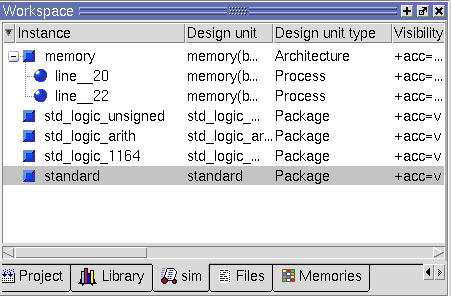
\includegraphics[width=.7\textwidth]{graficos/ms_mem1.png}
  \caption{Memoria compilada en Modelsim}
  \label{msmemsim}
\end{figure}

Luego, en la pestaña ``Memories'' se verá el arreglo (figura \ref{mem2})

\begin{figure}[h]
  \centering
    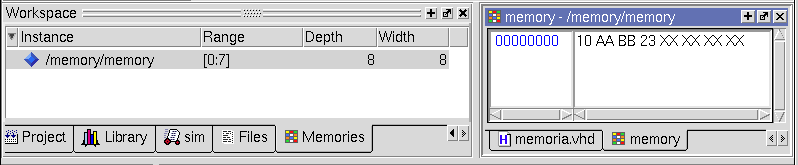
\includegraphics[width=1\textwidth]{graficos/ms_mem2.png}
  \caption{Carga y lectura de memoria en Modelsim}
  \label{mem2}
\end{figure}

Para importar o exportar datos a la memoria se utilizarán los archivos ``*.mem'' que tiene la
estructura de la figura \ref{mem3}

\begin{figure}[h]
  \centering
    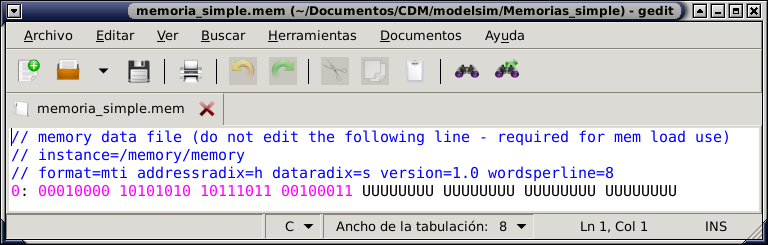
\includegraphics[width=1\textwidth]{graficos/ms_mem3.png}
  \caption{Estructura del archivo mem}
  \label{mem3}
\end{figure}

En la simulación de la figura \ref{mem4} se inicia con la memoria vacía, y se escriben los valores
``11110000'' en la dirección ``0x1'' y luego ``00001111'' en la dirección ``0x2''.

\begin{figure}[]
  \centering
    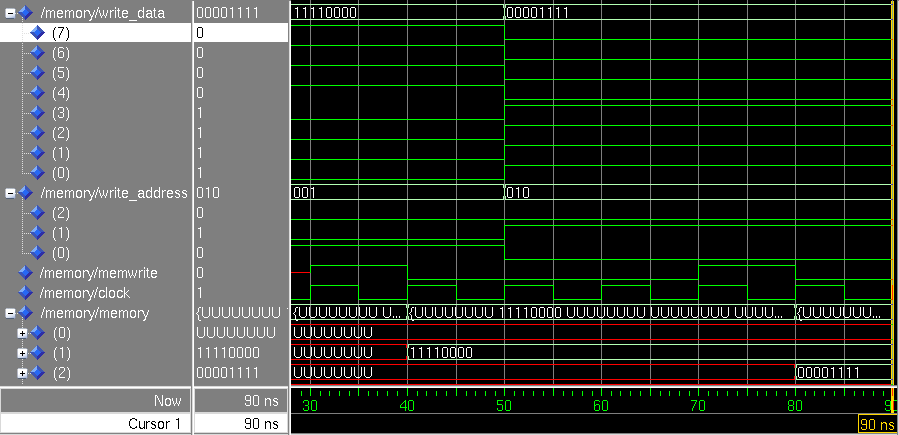
\includegraphics[width=1\textwidth]{graficos/write.png}
  \caption{Simulación del proceso de escritura}
  \label{mem4}
\end{figure}

Para simular la lectura, la memoria se inicializa con los valores de la tabla \ref{memlect}
\begin{table}[!ht] 
\centering
 \begin{tabular}{|c|c|c|c|c|c|c|c|c|}
\hline
\textbf{Dirección} & 0x0 & 0x1 & 0x2 & 0x3 & 0x4 & 0x5 & 0x6 & 0x7 \\ \hline
\textbf{Dato} & 0x00 & 0x0F & 0XF0 & 0xXX & 0xXX & 0xXX & 0xXX & 0xXX \\ \hline
\end{tabular}
  \caption{Inicialización de la memoria para simular lectura}
  \label{memlect}
\end{table}  

En la sumulación de la figura \ref{mem5} se leen las direcciones ``0x1'', ``0x2'', y ``0x0''.

\begin{figure}[]
  \centering
    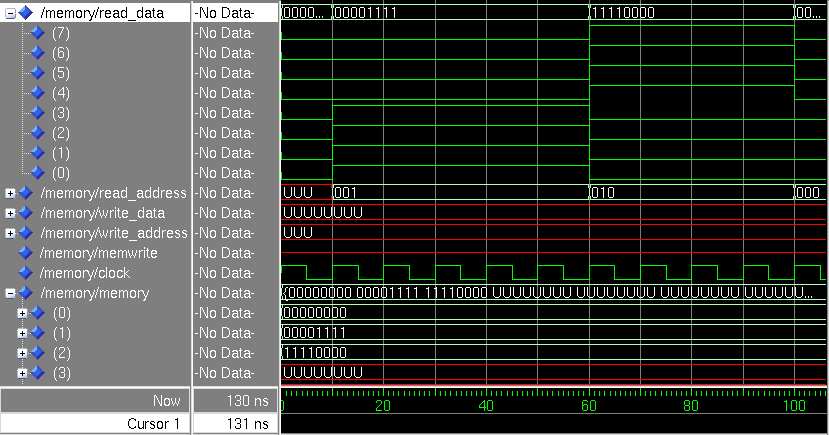
\includegraphics[width=1\textwidth]{graficos/read.png}
  \caption{Simulación del proceso de lectura}
  \label{mem5}
\end{figure}

\section{Microprocesador simple}
En esta sección se verá como interconectar los dispositivos vistos en la sección anterior para
realizar un microprocesador sencillo en VHDL. Para ello se describirá brevemente algunos conceptos
genéricos del microprocesador a implementar.

\subsection{Computadora sencilla}
Un diseño tradicional de la arquitectura interna de una computadora consiste en tres unidades 
principales, el procesador (CPU), las memorias donde guardar el programa y los datos, 
y un módulo de entrada salida para comunicarnos con el exterior.
La figura \ref{arquitectura} esquematiza estos tres módulos interconectados por dos buses
principales, uno de direcciones y otro de datos, adicionalmente existirán lineas de control 
para indicar el flujo de la información entre dichos módulos.

\begin{figure}[h]
  \centering
    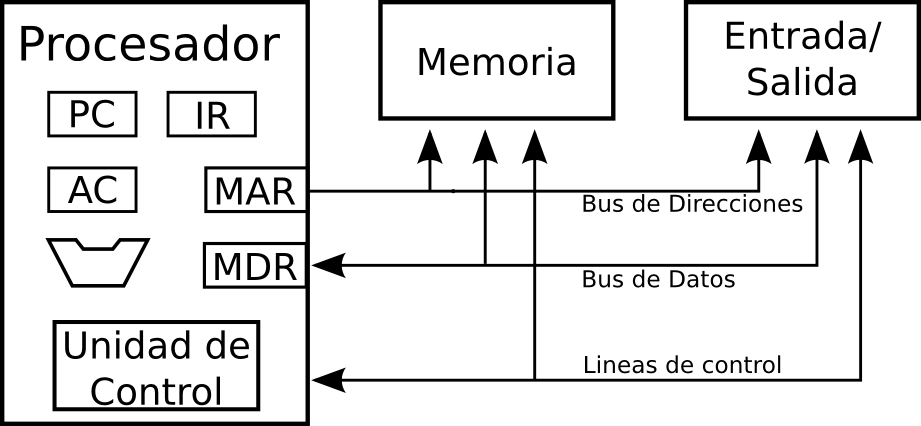
\includegraphics[width=.8\textwidth]{graficos/computadora.png}
  \caption{Arquitectura de una computadora simple}
  \label{arquitectura}
\end{figure}

Internamente el procesador contiene varios registros para almacenar datos dentro del
procesador. Algunos registros será visibles para el usuario como el Acumulador (AC) y el 
Program Counter (PC). Mientras que otros servirán para manejo interno:

\begin{itemize}
 \item MAR (Memory Addres Register): Este registro contiene la dirección del dato que se 
 quiere leer o escribir. El registro está conectado con el bus de direcciones, y su contenido se refleja en este bus.
 \item MDR (Memory Data Register): El registro está conectado al bus de datos y a través de él, 
 el CPU lee o escribe un dato a dicho bus.
 \item IR (Instruction Register): Después de que se ha obtenido una instrucción de la memoria, la CPU lo 
 almacena en este registro.
\end{itemize}

\subsection{Instrucciones y programas}
Para el desarrollo del microprocesador se define un formato de instrucción como el que se observa en 
la figura \ref{instruction}

\begin{figure}[h]
  \centering
    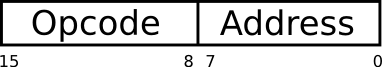
\includegraphics[width=.3\textwidth]{graficos/instruccion.png}
  \caption{Formato de la instrucción}
  \label{instruction}
\end{figure}

El set de instrucciones que implementaremos es básico (4 instrucciones), se describe en la tabla 
\ref{set_instruccion}

\begin{table}[!hbt] 
\centering
\begin{tabular}{|l|l|c|}
\hline
 \textbf{Mnemonico} & \textbf{Operación} & \textbf{OpCode}\\ \hline
ADD dirección & AC $\Leftarrow$ AC + contenido de la dirección de memoria & 00\\ \hline
STORE dirección& contenido de la dirección de memoria $\Leftarrow$ AC & 01\\ \hline
LOAD dirección& AC $\Leftarrow$ contenido de la dirección de memoria & 02\\ \hline
JUMP dirección& PC $\Leftarrow$ dirección & 03 \\ \hline
JNEG dirección& Si AC < 0 entonces PC $\Leftarrow$ dirección & 04 \\ \hline
\end{tabular}
  \caption{Set de instrucciones}
  \label{set_instruccion}
\end{table}

\subsection{Ciclos de ``Fetch'', ``Decode'', ``Execute''}
Normalmente las instrucciones se dividirán en varias etpas de instrucción, que llamaremos
``Fetch, Decode y Execute'' (F-D-E) respectivamente.
El ciclo F-D-E es el período que tarda un CPU en ejecutar una instrucción en código de máquina. 
El procesador captura (``fetch'') una instrucción de memoria, la decodifica (``decode``) 
para determinar que operando requiere y luego la ejecuta (''execute'').

La implementación del ciclo de F-D-E requiere algunas transferencias de registros y ciclos de reloj.

La figura \ref{fde} describe las acciones a realizar en cada etapa.

\begin{figure}[h]
  \centering
    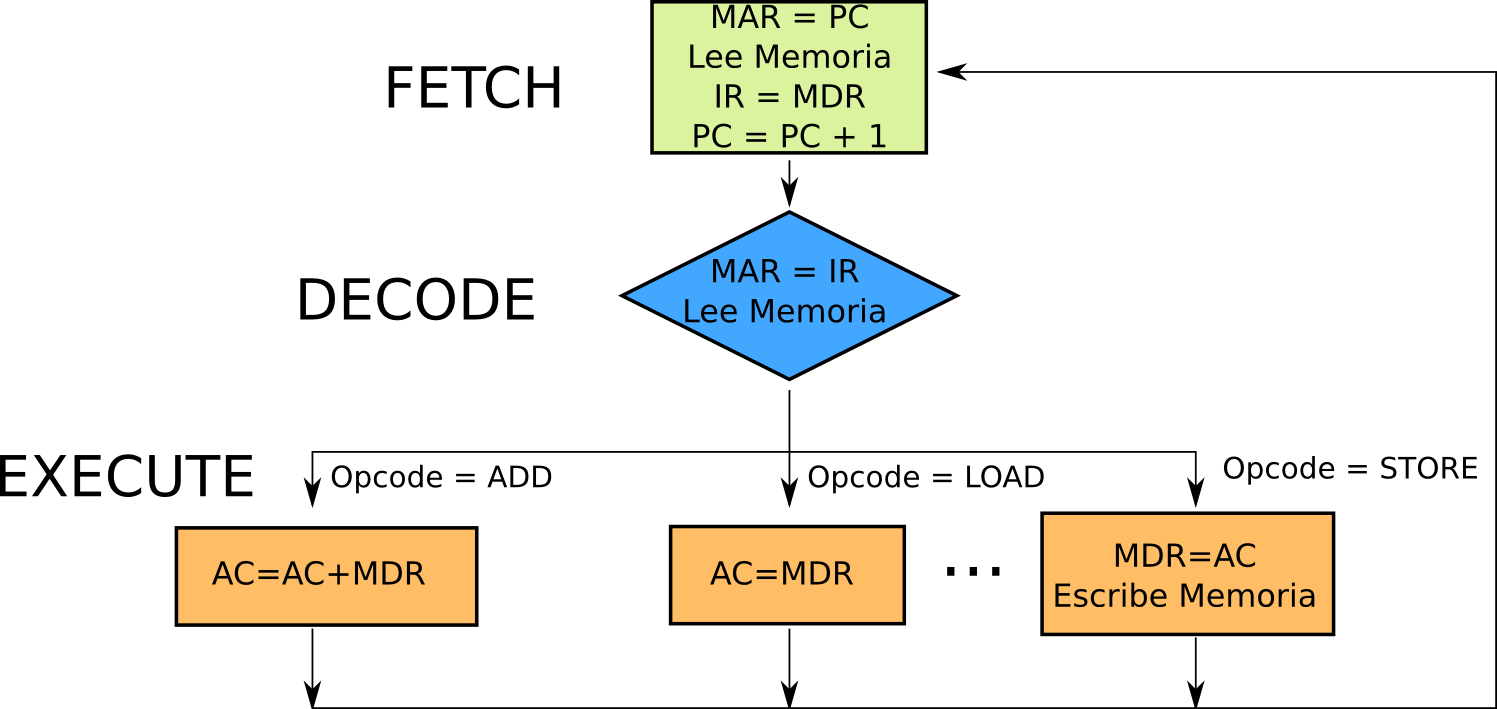
\includegraphics[width=1\textwidth]{graficos/fde.png}
  \caption{Ciclo de Fetch, Decode y Execute}
  \label{fde}
\end{figure} 

El ``Program Counter'' (PC) tiene la dirección de la instrucción actual. Normalmente para captar la próxima
instrucción de memoria el procesador deberá incrementar el PC. 
El registro de direcciones de memoria (MAR) se deberá actualizar con el PC de la instrucción que se captará.

\subsection{Modelo en VHDL}

memoria.vhd:
\begin{lstlisting}[style=vhdl, basicstyle=\footnotesize\ttfamily]
LIBRARY IEEE;
USE IEEE.STD_LOGIC_1164.ALL;
USE IEEE.STD_LOGIC_ARITH.ALL;
USE IEEE.STD_LOGIC_UNSIGNED.ALL;
ENTITY memory IS
  PORT( read_data     : OUT STD_LOGIC_VECTOR( 15 DOWNTO 0 );
        read_address  : IN STD_LOGIC_VECTOR( 7 DOWNTO 0 );
        write_data    : IN STD_LOGIC_VECTOR( 15 DOWNTO 0 ); 
        write_address : IN STD_LOGIC_VECTOR( 7 DOWNTO 0 );
        Memwrite      : IN STD_LOGIC;
        Clock         : IN STD_LOGIC );
  END memory;

ARCHITECTURE behavior OF memory IS
                --Define un nuevo tipo de datos de arreglo de memoria
  TYPE memory_type IS ARRAY ( 0 TO 255 ) OF STD_LOGIC_VECTOR( 15 DOWNTO 0 );
  SIGNAL memory: memory_type;
BEGIN
  --Lee la memoria y convierte el indice del arreglo a entero mediante CONV_INTEGER
  read_data <= memory( CONV_INTEGER( read_address( 7 DOWNTO 0 ) ) ) ;
  PROCESS       --Escritura de memoria
  BEGIN
    WAIT UNTIL clock 'EVENT AND clock = '1';
    IF ( memwrite = '1' ) THEN
                   --Convierte el indice del arreglo a entero mediante CONV_INTEGER
      memory( CONV_INTEGER( write_address( 7 DOWNTO 0 ) ) ) <= write_data;
    END IF;
  END PROCESS;
END behavior;
\end{lstlisting}

uprocesador.vhd:
\begin{lstlisting}[style=vhdl, basicstyle=\footnotesize\ttfamily]
LIBRARY IEEE;
USE IEEE.STD_LOGIC_1164.ALL;
USE IEEE.STD_LOGIC_ARITH.ALL;
USE IEEE.STD_LOGIC_UNSIGNED.ALL;

ENTITY SCOMP IS 
PORT( clock, reset  : IN STD_LOGIC;
      program_counter_out : OUT STD_LOGIC_VECTOR( 7 DOWNTO 0 );
      register_AC_out : OUT STD_LOGIC_VECTOR(15 DOWNTO 0 );
      memory_data_register_out : OUT STD_LOGIC_VECTOR(15 DOWNTO 0 ));
END SCOMP;

ARCHITECTURE up OF scomp IS
TYPE STATE_TYPE IS ( reset_pc, fetch, decode, execute_add, execute_load, 
execute_store, execute_store3, execute_store2, execute_jump );
SIGNAL state: STATE_TYPE;
SIGNAL instruction_register, memory_data_register : STD_LOGIC_VECTOR(15 DOWNTO 0 );
SIGNAL register_AC : STD_LOGIC_VECTOR(15 DOWNTO 0 );
SIGNAL program_counter : STD_LOGIC_VECTOR( 7 DOWNTO 0 );
SIGNAL memory_address_register : STD_LOGIC_VECTOR( 7 DOWNTO 0 );
SIGNAL memory_write : STD_LOGIC;

                      --Instanciacion de memoria (256 16-bit words)
  COMPONENT memory
    PORT( read_data     : OUT STD_LOGIC_VECTOR( 15 DOWNTO 0 );
          read_address  : IN STD_LOGIC_VECTOR( 7 DOWNTO 0 );
          write_data    : IN STD_LOGIC_VECTOR( 15 DOWNTO 0 ); 
          write_address : IN STD_LOGIC_VECTOR( 7 DOWNTO 0 );
          Memwrite      : IN STD_LOGIC;
          Clock         : IN STD_LOGIC );
  END COMPONENT;

  BEGIN
    memory_256: memory
           PORT MAP( read_data      => memory_data_register,
                     read_address   => memory_address_register,
                     write_data     => register_AC , 
                     write_address  => memory_address_register,
                     Memwrite       => memory_write,   
                     Clock          => clock);

    program_counter_out       <= program_counter;
    register_AC_out           <= register_AC;
    memory_data_register_out  <= memory_data_register;


                      --Estados

PROCESS ( CLOCK, RESET )
  BEGIN
  IF reset = '1' THEN
    state <= reset_pc;
  ELSIF clock'EVENT AND clock = '1' THEN
    CASE state IS
                  --Reseteo de la computadora, necesario para limpiar los registros                  
    WHEN reset_pc =>
        program_counter         <= "00000000";
        memory_address_register <= "00000000";
        register_AC             <= "0000000000000000";
        memory_write            <= '0';
        state                   <= fetch;
                  --Capta la instruccion de memoria y suma 1 al PC
    WHEN fetch =>
        instruction_register    <= memory_data_register;
        program_counter         <= program_counter + 1;
        memory_write            <= '0';
        state                   <= decode;        
                  --Decodifica la instruccion y envia la direccion del operando
    WHEN decode =>
        memory_address_register <= instruction_register( 7 DOWNTO 0);
        CASE instruction_register( 15 DOWNTO 8 ) IS
              WHEN "00000000" =>
                state <= execute_add;
              WHEN "00000001"=>
                state <= execute_store;
              WHEN "00000010" =>
                state <= execute_load;
              WHEN "00000011"=>
                state <= execute_jump;
              WHEN OTHERS =>
                state <= fetch;
        END CASE;
                  --Ejecuta la instruccion ADD
    WHEN execute_add =>
      register_ac             <= register_ac + memory_data_register;
      memory_address_register <= program_counter;
      state                   <= fetch;
                  --Ejecuta la instruccion STORE
                  --(necesita tres ciclos de clock)
    WHEN execute_store =>
      memory_write  <='1';
      state         <= execute_store2;
                  --Este estado asegura que la direccion de memoria
                  --es valida hasta despues que memory_write se desactiva
    WHEN execute_store2 =>
      memory_write  <= '0';
      state         <= execute_store3;
    WHEN execute_store3 =>  memory_address_register <= program_counter;
      state         <= fetch;
                  --Ejecuta la instruccion LOAD
    WHEN execute_load =>
      register_ac             <= memory_data_register;
      memory_address_register <= program_counter;
      state                   <= fetch;
                  --Ejecuta la instruccion JUMP
    WHEN execute_jump =>  
      memory_address_register <= instruction_register( 7 DOWNTO 0 );
      program_counter         <= instruction_register( 7 DOWNTO 0 );
      state                   <= fetch;
    WHEN OTHERS =>
      memory_address_register <= program_counter;
      state                   <= fetch;
    END CASE;
  END IF;
  END PROCESS;
END up;
\end{lstlisting}
\subsection{Simulaciones}
Para realizar la simulación, haremos un cálculo sencillo que se implementará en la memoria:


\lstset{language={[x86masm]Assembler}}
\begin{lstlisting}[basicstyle=\footnotesize\ttfamily]
 LOAD A  ;Cargo el primer valor de $11
 ADD B   ;Sumo el contenido de $11 a $12
 STORE C ;Guardo el resultado en $10
\end{lstlisting}
\lstset{language=vhdl}

Para cargar el programa en la memoria generaremos un archivo
binario con los opcodes del programa anterior e inicializaremos las
direcciones de memoria 0x11 y 0x12. El archivo ``memoria.mem'' 
quedará, por lo tanto, como se observa en la figura \ref{uprocmemoria}

\begin{figure}[h!]
  \centering
    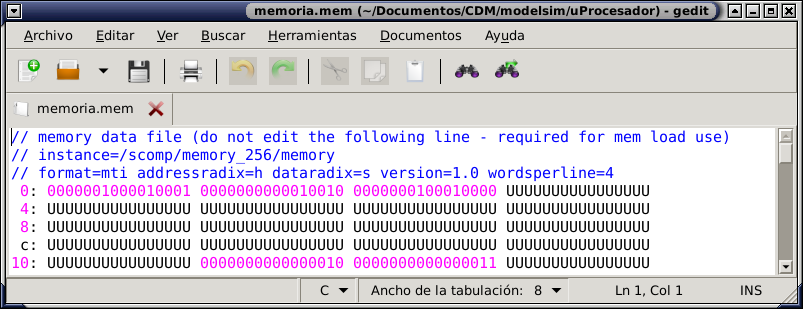
\includegraphics[width=1\textwidth]{graficos/memoria_uproc.png}
  \caption{Estructura del archivo ``memoria.mem''}
  \label{uprocmemoria}
\end{figure}

Como se observa en la simulación de la figura \ref{msuprocesador}, luego de que baja la señal de 
``Reset'', la señal ``State'' comienza con el estado ``reset'', luego pasa a ``Fetch'', ``Decode'' 
y ``Execute'' para las tres instrucciones. El program counter avanza de la posición ``0x00'' hasta
la ``0x03''. Cuando se produce el estado ``Execute\_store2'', se activa la señal de escritura en memoria.

\begin{figure}[h!]
  \centering
    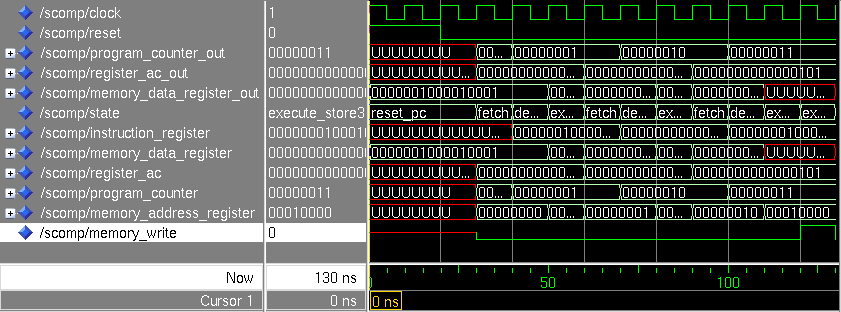
\includegraphics[width=1\textwidth]{graficos/uprocesador.png}
  \caption{Simulación del procesador}
  \label{msuprocesador}
\end{figure}

Luego de la ejecución del código la memoria queda con la información de la figura \ref{mempostsimulation}.

\begin{figure}[h!]
  \centering
    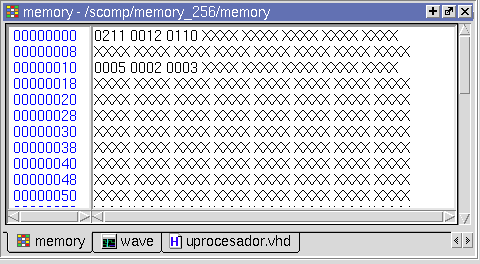
\includegraphics[width=.6\textwidth]{graficos/uprocpostsimulation.png}
  \caption{Estado de la memoria luego de la simulación}
  \label{mempostsimulation}
\end{figure}

\newpage

\subsection{Implementación}
A continuación se describirán algunos detalles de la implementación en la FPGA.

El procesador desarrollado hasta ahora es muy sensillo y no posee ninguna unidad de depuración para ingresar el código a depurar. Por lo
tanto a la hora de realizar la implementación, nos encontraremos con la dificultad de escribir el código en la memoria.

Herramientas como Quartus de Altera o ISE de Xilinx, poseen herramientas para inicializar directamente la memoria ram. Para utilizar estas herramientas 
necesitariamos implementar por lo menos un controlador de memoria.

Como el objetivo de este tutorial es implementar un procesador sensillo, se propone una solución de implementación que es independiente
del fabricante de FPGA (herramientas IDE) cómo de la arquitectura del circuito que se utilizará.
La técnica consiste en preinicializar sectores del vector de memoria con los valores que se desean escribir de la siguiente manera:

memoria.vhd:
\begin{lstlisting}[style=vhdl, basicstyle=\footnotesize\ttfamily]

  PROCESS       --Escritura de memoria
  BEGIN
  process(reset,clock,memwrite) begin
    if reset='1' then
	  memory(0) <= x"0211";
	  memory(1) <= x"0012";
	  memory(2) <= x"0110";
	  memory(3) <= x"0302";
	  memory(11) <= x"0002";
	  memory(12) <= x"0003";
     for i in 13 to 255 loop 
	    memory(i) <= x"0000";
		 end loop;
  .....
  end process;
\end{lstlisting}


%\section{Modelsim}
%Completar
\section{Bibliografía}
\small{
[1] ``Rapid Prototyping of Digital Systems'', Sec. Edition, James O. Hamblen, M. Furmman

[2] ``Digital Design, Principles \& Practices'', Third Edition, John F. Walkerly.

[3] ``DE0 User Manual'', Altera.

[4] ``ModelSim User's Manual'', Mentor Graphics
}
\end{document}
